\section{Process Fidelity Eval}

Process Fidelity Eval measures whether goal progress follows a credible multi-agent process. A run succeeds only when the desired outcome and the required evidence chain are both satisfied. For a relationship goal, that evidence chain may include shared events, subjective memories for both agents, relationship-edge source references, and a later decision that cites a relevant memory or relationship edge.

\begin{figure}[t]
\centering
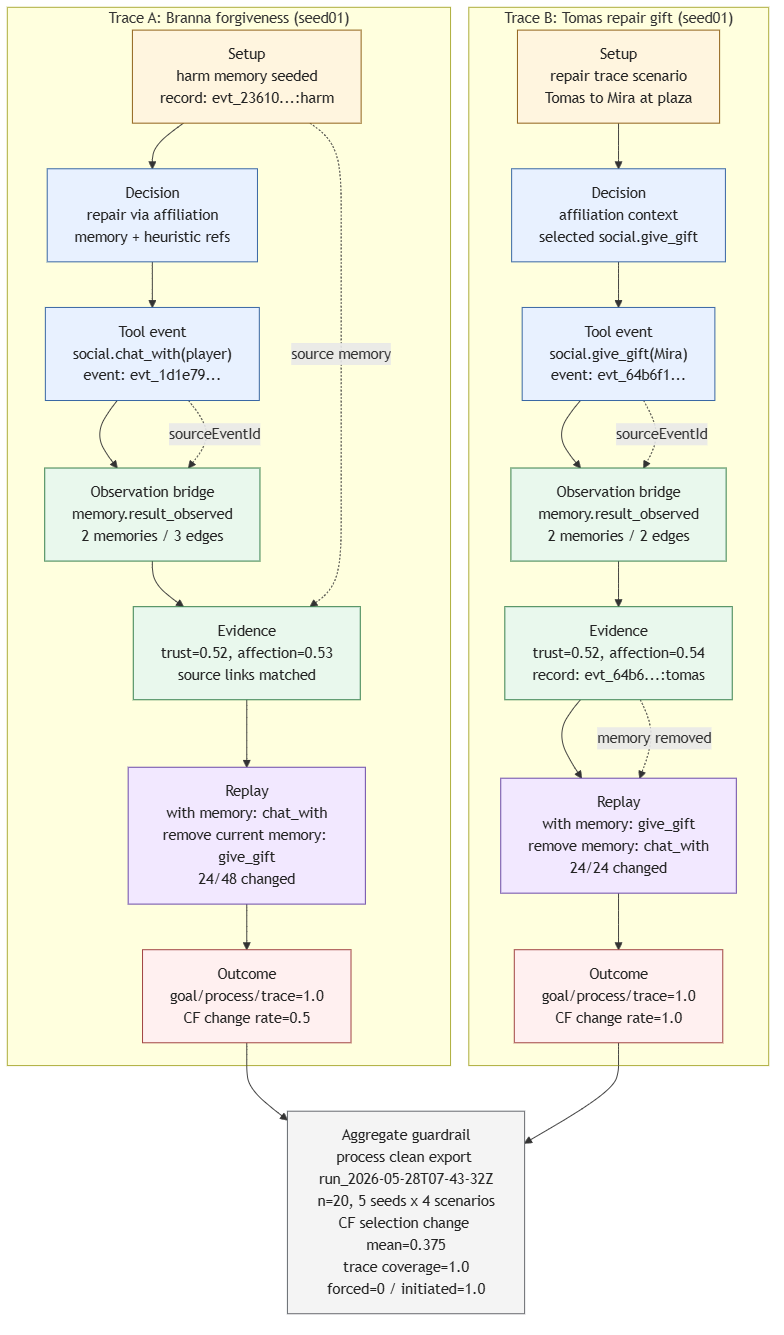
\includegraphics[width=\linewidth,height=0.72\textheight,keepaspectratio]{../generated/figures/trace_evidence_chain_figure3.png}
\caption{Trace evidence chains for two process-fidelity examples from the current clean process export, with an aggregate process-suite guardrail annotation. The editable Mermaid source at \texttt{paper/diagrams/trace\_evidence\_chain\_figure3.mmd} uses curated labels from process artifacts rather than raw event-summary text.}
\label{fig:trace-evidence-chain}
\end{figure}

\begin{table}[t]
\centering
\small
\caption{Process Fidelity metric families used by the current draft.}
\label{tab:metric-families}
\begin{tabular}{lll}
\toprule
Family & Example metrics & Question answered \\
\midrule
Outcome & goal success, milestones & Did the run satisfy the stated goal evidence? \\
Process & process coverage, shortcuts & Did the required path occur without illegal jumps? \\
Autonomy & forced action, agent initiation & Did NPC arbitration choose the relevant actions? \\
Memory & causal use, ablation delta & Did remembered events affect later decisions? \\
Trace & trace coverage, source links & Can the causal chain be replayed from artifacts? \\
Side effects & spillover, overreach & Did intervention cause uncontrolled collateral change? \\
\bottomrule
\end{tabular}
\end{table}

The current baseline matrix includes Full Motivational Delegation, Hard Delegation, No Subjective Memory, No Relationship Edge, Shuffled Memory Owner, and Evidence-Link Removal. Hard Delegation represents the explicit worker-agent pattern: a Director decomposes the goal into assigned subtasks and gives them to specific NPCs. The memory and evidence-link ablations test whether relationship memory is causally useful, whether the correct owner of a memory matters, and whether traces still justify relationship changes after source links are removed.

All current exported results should be read as scaffolding evidence. The metrics are already wired to manifests and generated paper tables, yet stronger research claims need repeated seeds, LLM-backed provider runs, runtime-level ablations, and human process-believability ratings.
